\section{Users' Experience and Fraud on Bikroy.com}
\label{sec:users}

Section~\ref{sec:history} showed that Bikroy remains large but has never solved its trust
problem. This section examines what buyers and sellers actually experience on Bikroy,
whether people are still being scammed, and where exactly in a transaction the platform
leaves them exposed. We separate two things that are often
confused: how users rate the \emph{app} as a tool, and how safe a \emph{transaction} made
through it is.

\subsection{What users say}

\paragraph{The app itself is well liked.} It would be misleading to claim users hate Bikroy.
On Google Play, the Bikroy app has a 4.3-star average from about 210{,}000 reviews and more
than 10~million downloads (Figure~\ref{fig:ratings})~\cite{play_store}. People value it as a
fast way to post an ad and reach buyers. The most visible recent reviews (May--September
2026) complain mainly about usability after the switch to Jiji's platform: users report that
the redesigned interface is harder to navigate and that the filter separating member
(business) ads from individual sellers was removed, making person-to-person deals and price
comparison harder~\cite{play_store}.

\paragraph{Sellers who pay are less satisfied.} On Trustpilot, Bikroy scores 2.0 out of 5
from 13 reviews~\cite{trustpilot}. One seller advised others never to pay for ads, suspecting
that paid promotions trigger automated messages that only look like buyer interest; the same
reviewer objected to manual review and requests for private information on a flat-rental
ad~\cite{trustpilot}. Thirteen reviews is far too few to represent all users, so we treat
these as illustrative complaints rather than a measurement.

\begin{figure}[H]
  \centering
  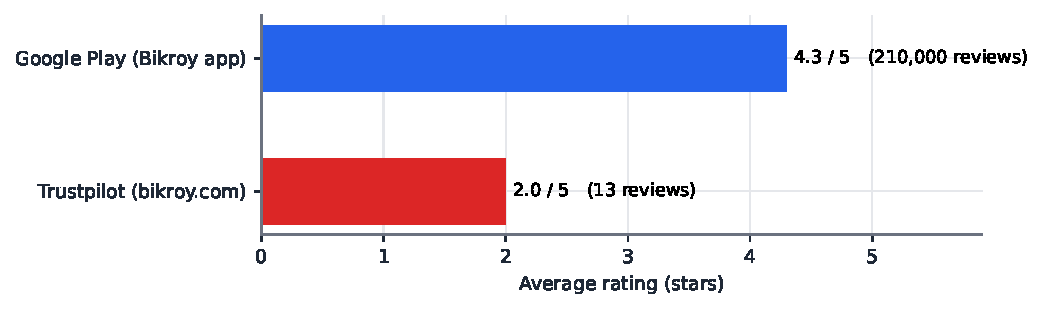
\includegraphics[width=0.85\textwidth]{fig7_ratings.pdf}
  \caption{Bikroy's ratings on two review platforms, as of October 2026. The very different
  sample sizes mean the two numbers measure different things: app usability for a large
  general audience versus experiences of a small, self-selected group.
  Sources: \cite{play_store,trustpilot}.}
  \label{fig:ratings}
\end{figure}

\paragraph{Why ratings do not measure safety.} A high app rating and a high scam risk can
coexist. App-store reviews are written mostly by people for whom the app worked; a buyer who
loses money to a fake seller blames the seller or the police process, not the app's
interface. National data show how rarely fraud victims take formal action at all: in a
2023--24 survey of 132 cybercrime victims by the Cyber Crime Awareness Foundation (CCAF),
40.15\% had suffered financial loss, but only 12\% pursued legal action
(Figure~\ref{fig:ccaf})~\cite{ccaf_2024}. Most fraud, in other words, is never recorded
anywhere a researcher can find it.

\begin{figure}[H]
  \centering
  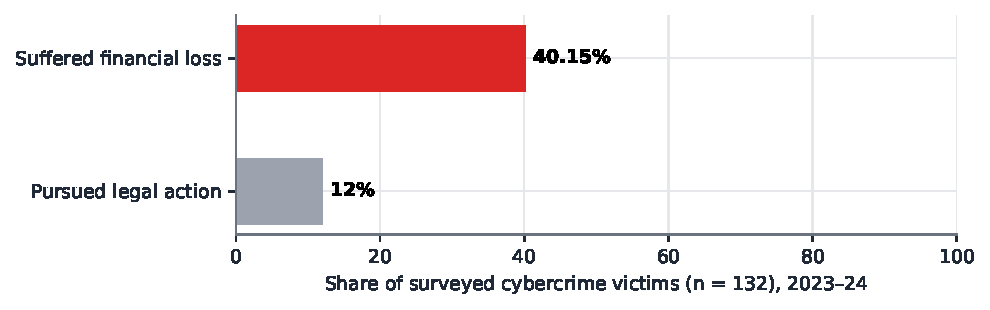
\includegraphics[width=0.85\textwidth]{fig8_ccaf.pdf}
  \caption{Financial loss versus legal action among 132 surveyed cybercrime victims in
  Bangladesh (survey period April 2023 -- April 2024). Source: CCAF~\cite{ccaf_2024}.}
  \label{fig:ccaf}
\end{figure}

\subsection{Documented scams and how they work}

Police and newspaper reports describe a small number of recurring scam patterns on Bikroy.
Table~\ref{tab:scams} classifies them by who is harmed and at which stage of the
transaction.

\begin{table}[H]
  \centering
  \small
  \caption{Scam patterns documented on Bikroy.com.}
  \label{tab:scams}
  \begin{tabularx}{\textwidth}{@{}>{\raggedright\arraybackslash}p{2.7cm} >{\raggedright\arraybackslash}p{1.3cm} >{\raggedright\arraybackslash}p{1.9cm} Y@{}}
    \toprule
    \textbf{Pattern} & \textbf{Victim} & \textbf{Stage} & \textbf{Evidence} \\
    \midrule
    Fake seller, advance payment & Buyer & Payment
      & Muktagacha gang posted cheap phone and electronics ads from accounts opened with
        SIM cards bought for Tk~350--500; took lakhs of taka~\cite{ds_muktagacha}.
        Fake sellers typically underprice items~\cite{dt_2014}. \\
    Lure and robbery & Buyer & Handover
      & In 2014 Bikroy itself reported fake sellers luring buyers to remote places and
        robbing them~\cite{dt_2014}. \\
    Fake buyer, counterfeit or swapped cash & Seller & Payment and handover
      & 2023: gang paid an iPhone seller with a bundle of mostly Tk~20 notes; active for
        more than three years; three arrested~\cite{pa_2023}. \\
    Fake or replica goods & Buyer & Listing
      & Widespread allegations by 2017 led Bikroy to ban replica and clone
        items~\cite{fs_fraud}. \\
    Fake inquiries after paid promotion & Seller & Listing
      & Seller complaint that paid ads attract automated, non-genuine
        messages~\cite{trustpilot} (unverified, single review). \\
    \bottomrule
  \end{tabularx}
\end{table}

Two of these patterns are traced step by step below. Figure~\ref{fig:advance} shows the
fake-seller scam as reconstructed from the Muktagacha case and Bikroy's own 2014 account.
Each check Bikroy runs (phone verification and ad review) happens \emph{before} the scam
starts; once buyer and seller are talking directly, the money moves entirely outside the
platform, and afterwards Bikroy's terms state that it is not a party to the
transaction~\cite{bikroy_terms}.

\begin{figure}[H]
  \centering
  \resizebox{0.97\textwidth}{!}{% Fake-seller / advance-payment scam, compiled from documented cases
\begin{tikzpicture}[
  font=\footnotesize,
  actor/.style={draw=ink, fill=#1!15, rounded corners=2pt, minimum width=2.6cm,
                minimum height=0.75cm, font=\footnotesize\bfseries},
  life/.style={draw=muted, densely dotted},
  msg/.style={-{Stealth[length=2mm]}, thick, draw=#1},
  lab/.style={font=\scriptsize, fill=white, inner sep=1.5pt, align=center}]

  \node[actor=bad]   (S) at (0,0)   {Scammer};
  \node[actor=muted] (B) at (5.2,0) {Bikroy};
  \node[actor=good]  (V) at (10.4,0){Buyer};
  \foreach \n in {S,B,V}{ \draw[life] (\n.south) -- ++(0,-8.1); }

  % 1
  \node[lab, anchor=west, text width=4.4cm] at (0.15,-1.0)
    {\textbf{1.} Buys registered SIM cards (Tk 350--500 each) and opens e-mail accounts};
  % 2
  \draw[msg=bad] (0,-1.9) -- node[lab, above]{\textbf{2.} Posts ad: phone/electronics far below market} (5.2,-1.9);
  % 3
  \draw[msg=muted] (5.2,-2.7) -- node[lab, above]{\textbf{3.} SMS-OTP passes; ad reviewed and published} (0,-2.7);
  % 4
  \draw[msg=muted] (5.2,-3.5) -- node[lab, above]{\textbf{4.} Ad shown to buyers} (10.4,-3.5);
  % 5
  \draw[msg=good] (10.4,-4.3) -- node[lab, above]{\textbf{5.} Contacts seller directly (phone)} (0,-4.3);
  % 6
  \draw[msg=bad] (0,-5.1) -- node[lab, above]{\textbf{6.} Asks for payment before sending the item} (10.4,-5.1);
  % 7
  \draw[msg=good] (10.4,-5.9) -- node[lab, above]{\textbf{7.} Pays in advance --- \emph{off-platform}} (0,-5.9);
  % 8
  \node[lab, anchor=west, text width=4.4cm, text=bad] at (0.15,-6.75)
    {\textbf{8.} Item never delivered; money kept (Tk lakhs across victims)};
  % 9
  \draw[msg=good, densely dashed] (10.4,-7.5) -- node[lab, above]{\textbf{9.} Reports: Bikroy is ``not a party''; liability capped} (5.2,-7.5);

  % bracket: Bikroy never touches the money
  \draw[decorate, decoration={brace, amplitude=5pt, mirror}, thick, bad]
    (10.9,-4.0) -- (10.9,-8.0)
    node[midway, right=7pt, font=\scriptsize, text=bad, align=left, text width=1.6cm]
    {Money moves with no platform control};
\end{tikzpicture}
}
  \caption{Typical fake-seller (advance-payment) scam on a classifieds platform, compiled
  from the Muktagacha case~\cite{ds_muktagacha}, Bikroy's 2014 statement~\cite{dt_2014} and
  Bikroy's current terms~\cite{bikroy_terms}. Steps 3--4 are the only points at which the
  platform is involved.}
  \label{fig:advance}
\end{figure}

Figure~\ref{fig:noteswap} shows the reverse case, where the \emph{seller} is the victim.
This scam does not need a fake listing at all: it exploits the cash meeting that Bikroy's
own safety advice recommends (meet in person, inspect, then pay)~\cite{bikroy_safety}.

\begin{figure}[H]
  \centering
  \resizebox{0.97\textwidth}{!}{% Fake-buyer counterfeit/note-swap scam (Prothom Alo, 2023)
\begin{tikzpicture}[
  font=\footnotesize, node distance=3mm,
  step/.style={draw=#1, fill=#1!10, rounded corners=2pt, text width=2.55cm,
               minimum height=1.55cm, align=center, font=\scriptsize},
  flow/.style={-{Stealth[length=2mm]}, thick, draw=ink}]

  \node[step=good]                 (a) {\textbf{1. Listing}\\Seller posts iPhone~13 on Bikroy at Tk~81,000};
  \node[step=muted, right=of a]    (b) {\textbf{2. Deal}\\``Buyer'' calls; price agreed at Tk~75,000};
  \node[step=muted, right=of b]    (c) {\textbf{3. Meetup}\\Three men meet seller outside a market in Mouchak};
  \node[step=bad, right=of c]      (d) {\textbf{4. Count}\\Seller counts a bundle of Tk~1,000 notes: correct};
  \node[step=bad, below=7mm of d]  (e) {\textbf{5. Swap}\\Bundle taken back ``for a rubber band'', swapped in seconds};
  \node[step=bad, left=of e]       (f) {\textbf{6. Loss}\\Inside: old Tk~20 notes. Phone gone; noticed only later, paying a restaurant bill};
  \node[step=muted, left=of f]     (g) {\textbf{7. Recourse}\\Police case at Ramna; DB arrests 3 (gang active 3+ years)};
  \node[step=good, left=of g, draw=good, fill=good!10, densely dashed]
                                   (h) {\textbf{With escrow}\\no cash changes hands: nothing to count, nothing to swap};

  \draw[flow] (a) -- (b); \draw[flow] (b) -- (c); \draw[flow] (c) -- (d);
  \draw[flow] (d) -- (e); \draw[flow] (e) -- (f); \draw[flow] (f) -- (g);
\end{tikzpicture}
}
  \caption{The 2023 note-swap scam against a seller who listed an iPhone~13 on Bikroy,
  reconstructed from Prothom Alo's report of the Detective Branch case~\cite{pa_2023}. The
  dashed box shows what an escrow payment would remove.}
  \label{fig:noteswap}
\end{figure}

\subsection{Where Bikroy's protection stops}

Putting the cases together gives a clear picture (Figure~\ref{fig:lifecycle}). A used-goods
deal passes through six stages. Bikroy has weak control over the first three (identity,
listing, contact) and none over the last three (payment, handover, dispute). The most
damaging documented scams (fake sellers, robbery and counterfeit cash) strike in the three
stages Bikroy does not control, while fake identities and replica goods pass through the weak
checks at the start.

\begin{figure}[H]
  \centering
  \resizebox{\textwidth}{!}{% Where Bikroy's protection stops along a used-goods transaction
\begin{tikzpicture}[
  font=\footnotesize,
  stage/.style={draw=ink, fill=white, rounded corners=2pt, minimum width=2.15cm,
                minimum height=0.9cm, align=center, font=\footnotesize\bfseries},
  cover/.style={rounded corners=2pt, minimum width=2.15cm, minimum height=1.25cm,
                align=center, text width=2.0cm, font=\scriptsize},
  hit/.style={draw=bad, fill=bad!8, rounded corners=2pt, align=center,
              font=\scriptsize, inner sep=3pt},
  flow/.style={-{Stealth[length=2mm]}, draw=ink, thick}]

  % stages
  \foreach \i/\name in {1/Identity, 2/Listing, 3/Contact \&\\negotiation,
                        4/Payment, 5/Handover, 6/Dispute \&\\recourse}{
    \node[stage] (s\i) at ({(\i-1)*2.45},0) {\name};
  }
  \foreach \a/\b in {1/2,2/3,3/4,4/5,5/6}{ \draw[flow] (s\a) -- (s\b); }

  % Bikroy's coverage at each stage
  \node[cover, fill=partial!25] (c1) [below=0.35cm of s1] {Phone OTP only\\(2017)};
  \node[cover, fill=partial!25] (c2) [below=0.35cm of s2] {Ad review before\\publishing};
  \node[cover, fill=partial!25] (c3) [below=0.35cm of s3] {In-app chat\\or phone call};
  \node[cover, fill=bad!22]     (c4) [below=0.35cm of s4] {\textbf{None}: cash or\\mobile money,\\off-platform};
  \node[cover, fill=bad!22]     (c5) [below=0.35cm of s5] {\textbf{None}: meet in\\person; ``Buy Now''\\on few listings};
  \node[cover, fill=bad!22]     (c6) [below=0.35cm of s6] {\textbf{None}: ``not a\\party''; liability\\$\le$ BDT 6,700};

  \node[anchor=east, font=\scriptsize\itshape, text=muted, align=right]
    at ([xshift=-2pt]c1.west) {Bikroy\\covers};

  % where documented scams strike
  \node[hit, text width=4.4cm] (h1) at ($(c1.south)!0.5!(c2.south)+(0,-1.0)$)
    {Fake identity: SIMs bought for Tk 350--500 pass OTP; one in three ads not genuine (2014)};
  \node[hit, text width=1.95cm] (h2) at ($(c4.south)+(0,-1.15)$)
    {Advance paid to fake seller is lost};
  \node[hit, text width=1.95cm] (h3) at ($(c5.south)+(0,-1.15)$)
    {Robbery at meetup; counterfeit-cash swap};
  \node[hit, text width=1.95cm] (h4) at ($(c6.south)+(0,-1.15)$)
    {Victim's only route: police case};
  \foreach \h/\c in {h1/c1,h1/c2,h2/c4,h3/c5,h4/c6}{
    \draw[-{Stealth[length=1.6mm]}, bad, densely dashed] (\h.north) -- (\c.south);
  }
  \node[anchor=east, font=\scriptsize\itshape, text=bad, align=right]
    at ([xshift=-2pt]h1.west) {Documented\\scams};

  % legend
  \node[draw=partial, fill=partial!25, minimum width=3mm, minimum height=3mm] (l1) at (3.4,-5.25) {};
  \node[right=1mm of l1, font=\scriptsize] {weak, partial control};
  \node[draw=bad, fill=bad!22, minimum width=3mm, minimum height=3mm] (l2) at (7.3,-5.25) {};
  \node[right=1mm of l2, font=\scriptsize] {no platform control};
\end{tikzpicture}
}
  \caption{Bikroy's control over each stage of a used-goods transaction (orange: weak or
  partial; red: none), and where the documented scams in Table~\ref{tab:scams} strike.
  Sources: \cite{fs_fraud,ds_jiji,bikroy_terms,bikroy_safety,ds_muktagacha,dt_2014,pa_2023}.}
  \label{fig:lifecycle}
\end{figure}

\subsection{Are people still being scammed in 2026?}
\label{sec:still}

We should be precise about what the evidence shows.

\begin{itemize}
  \item \textbf{Bikroy-named cases.} The police cases we found that explicitly name Bikroy
  run up to 2023~\cite{pa_2023,ds_muktagacha}. We did not find a 2025--26 news report that
  names Bikroy, but newspapers often describe the platform only as ``online'', so this is
  absence of reporting, not evidence that the scams stopped.
  \item \textbf{The platform's own position.} In 2026 every Bikroy listing still carries
  warnings to avoid advance payment and to meet in a public place~\cite{bikroy_listing}, and
  its terms still disclaim responsibility for losses between users~\cite{bikroy_terms}. The
  conditions that made these scams possible are unchanged.
  \item \textbf{The same pattern elsewhere.} Advance-payment fraud through online ads is
  still being prosecuted in 2026: in August 2026, police in Narail arrested members of a
  gang that took money through online ads for hilsa fish and recovered phones, SIM cards and
  Tk~60{,}000~\cite{itv_hilsa}.
\end{itemize}

\subsection{The national lesson: escrow already works}
\label{sec:escrowlesson}

Advance-payment fraud is not unique to Bikroy; it is one of the defining failures of
Bangladeshi online commerce. Evaly, which sold goods at half price against advance payment and then
failed to deliver, owed about Tk~543 crore to customers and suppliers; its founders were
sentenced in January 2025~\cite{bdnews_evaly}. A similar case against e-Orange was still
in court in February 2026~\cite{bdnews_eorange}.

The government's response was escrow. On 30~June~2021 Bangladesh Bank issued a circular
requiring payment gateways to hold customers' advance payments and release them to the
merchant only after the product is delivered and the delivery documents are
verified~\cite{tbs_escrow}. The effect was measurable (Figure~\ref{fig:escrow}): of
Tk~5.05~billion that customers paid through gateways from 14~October~2021, Tk~2.14~billion
was still being held when the failed platforms collapsed, and in October 2021 the government
decided to return it to customers who had not received their goods~\cite{fe_refund}.

\begin{figure}[H]
  \centering
  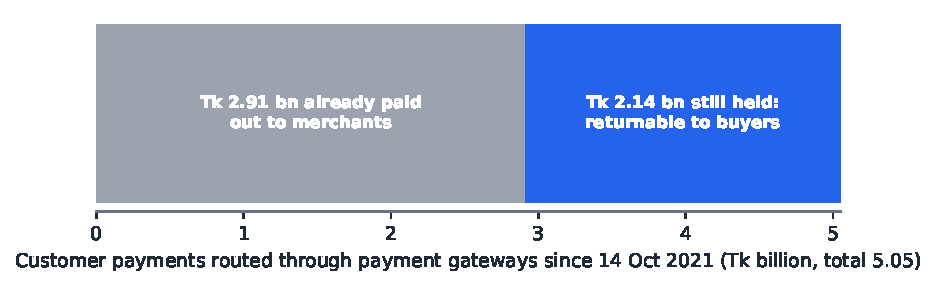
\includegraphics[width=0.9\textwidth]{fig9_escrow_funds.pdf}
  \caption{Customer payments routed through payment gateways under the 2021 escrow system,
  split into money already released to merchants and money still held, which could be
  returned to buyers. Source: The Financial Express~\cite{fe_refund}.}
  \label{fig:escrow}
\end{figure}

This regime protects buyers of \emph{business} e-commerce sites. It does not reach
person-to-person deals arranged through classifieds, because on Bikroy the payment never
passes through the platform or a gateway at all: buyer and seller settle in cash or by
direct transfer~\cite{bikroy_terms}. The protection Bangladesh already decided online buyers
need therefore stops exactly where individual resale begins.

\subsection{Summary: the loopholes}
\label{sec:loopholes}

The evidence in Sections~\ref{sec:history} and~\ref{sec:users} identifies six loopholes,
which Section~\ref{sec:solution} maps to TrustBazaar's features.

\begin{enumerate}[label=\textbf{L\arabic*.}]
  \item \textbf{Weak identity.} A phone number is the only identity check, and registered SIM
  cards can be bought for Tk~350--500~\cite{fs_fraud,ds_muktagacha}.
  \item \textbf{No payment protection.} Money moves off-platform with no holding
  point~\cite{bikroy_terms,bikroy_safety}.
  \item \textbf{Unsafe handover.} Buyers and sellers must meet with cash, which enables
  robbery and counterfeit-cash swaps~\cite{dt_2014,pa_2023}.
  \item \textbf{No recourse.} Bikroy is not a party to the deal, caps its liability at
  BDT~6{,}700 and offers no dispute process~\cite{bikroy_terms}.
  \item \textbf{No accountability record.} There is no verified transaction history, so a
  scammer can return under a new number, and Bikroy has published no fraud measurement since
  2014~\cite{dt_2014}.
  \item \textbf{No fair price discovery.} Bikroy offers fixed prices and informal
  negotiation only; there is no auction format with enforced rules.
\end{enumerate}
